\section{Brief Introduction to Quantum Computation}

Computations, regardless of how it is performed, at its most fundamental level is a physical process. 
Human perform computations in our mind by the biochemical process that took place in the brain, classical computer by transmitting electronic signals in the circuit boards, and \textit{quantum computers} by manipulating and measuring  the states of quantum mechanical objects.

The following postulates of quantum mechanics is key to our discussions
\begin{enumerate}[label={\textbf{Postulate} \arabic*}]
	\item the simplest quantum state is \textit{qubit}, which is described by unit vector in $\mathbb{C}^2$;
	\item composition of $n$-qubit state is described by unit vector in $(\mathbb{C}^2)^{\otimes n} \cong \mathbb{C}^{2^n}$;
	\item states evolved by unitary\footnote{$U$ is unitary if $U^\dagger U = I$} operations.
	\item quantum measurement is governed by the Born rule.
\end{enumerate}

We will dicuss the first three postulates here, while leaving the discussion of Born rule to section \ref{sec:measurement}.

Let $\ket{1} = \begin{pmatrix}1 \\ 0\end{pmatrix}$ and $\ket{0} = \begin{pmatrix}0 \\ 1\end{pmatrix}$ be the standard orthonormal basis of $\mathbb{C}^2$.
Any one qubit state $\ket{\psi}$, therefore, can be described as 
$$
\ket{\psi} = a\ket{0} + b\ket{1}, \quad a, b \in \mathbb{C}, |a|^2 + |b|^2 = 1
$$

The following unitary operators are called Pauli operators, which will be important for later discussions and are presented here as examples of unitaries operations.
\begin{equation}\label{eq:pauli}
	X = \begin{pmatrix}
0 & 1\\
1 & 0
\end{pmatrix}, \quad Y = \begin{pmatrix}0 & -i\\
i & 0
\end{pmatrix}, \quad Z = \begin{pmatrix}1 & 0\\
0 & -1
\end{pmatrix}
\end{equation}

It is worth discussing why states evolve according to unitary matrices.
The time evolution of a closed quantum state $\ket{\psi}$ is described by the \textit{Schrödinger equation}

\begin{equation}\label{schrodinger}
	i \hslash \frac{d \ket{\psi}}{d t} = H \ket{\psi}
\end{equation}
If $H$ is a time independent Hamiltonian, the solution \eqref{schrodinger} is 
$$
\ket{\psi(t)} = e^{\frac{-iH t}{\hslash}} \ket{\psi(0)}
$$
where $\ket{\psi(0)}$ is the initial state of the system.
Standard results from linear algebra show that for Hermitian $H$, $e^{\frac{-i H t}{\hslash}}$ is indeed unitary for any real $t$.

The existence of qubit systems in nature has been demonstrated by the famous Stern-Gerlach experiment \cite{Sakurai_Napolitano_2020}. 
Various physical realisations of quantum computers have been proposed, such as those based on ion traps \cite{steane1997ion}, optical photon \cite{gardiner2004quantum}, and nuclear magnetic resonance \cite{nmr} among others.

In this article we will regard qubit and its unitary evolution as our fundamental quantum mechanical system and describe the theories of unitary operation.

\subsection{Single Qubit Operation}

The Bloch sphere representation of a qubit is very helpful for our discussion.
Any qubit $\ket{\psi}$ can be written $\ket{\psi} = a \ket{0} + b \ket{1}$ for some $a , b \in \mathbb{C}$ such that $|a|^2 + |b|^2 = 1$.
If we write $|a| = \cos \frac{\theta}{2}$ and $|b| = \sin \frac{\theta}{2}$, then for some phase factors $e^{i \alpha}$ and $e^{i \beta}$, we have
$$
\ket{\psi} = e^{i \beta} \left(\cos \frac{\theta}{2} \ket{0} + e^{i \alpha} \sin \frac{\theta}{2} \ket{1}\right),
$$

We can represent $\ket{\psi}$ as a point on the unit sphere, where $\theta$ and $\alpha$ denote the polar and azimuthal angles. 
This is called a Bloch sphere.

\begin{figure}[htbp]
	\centering
	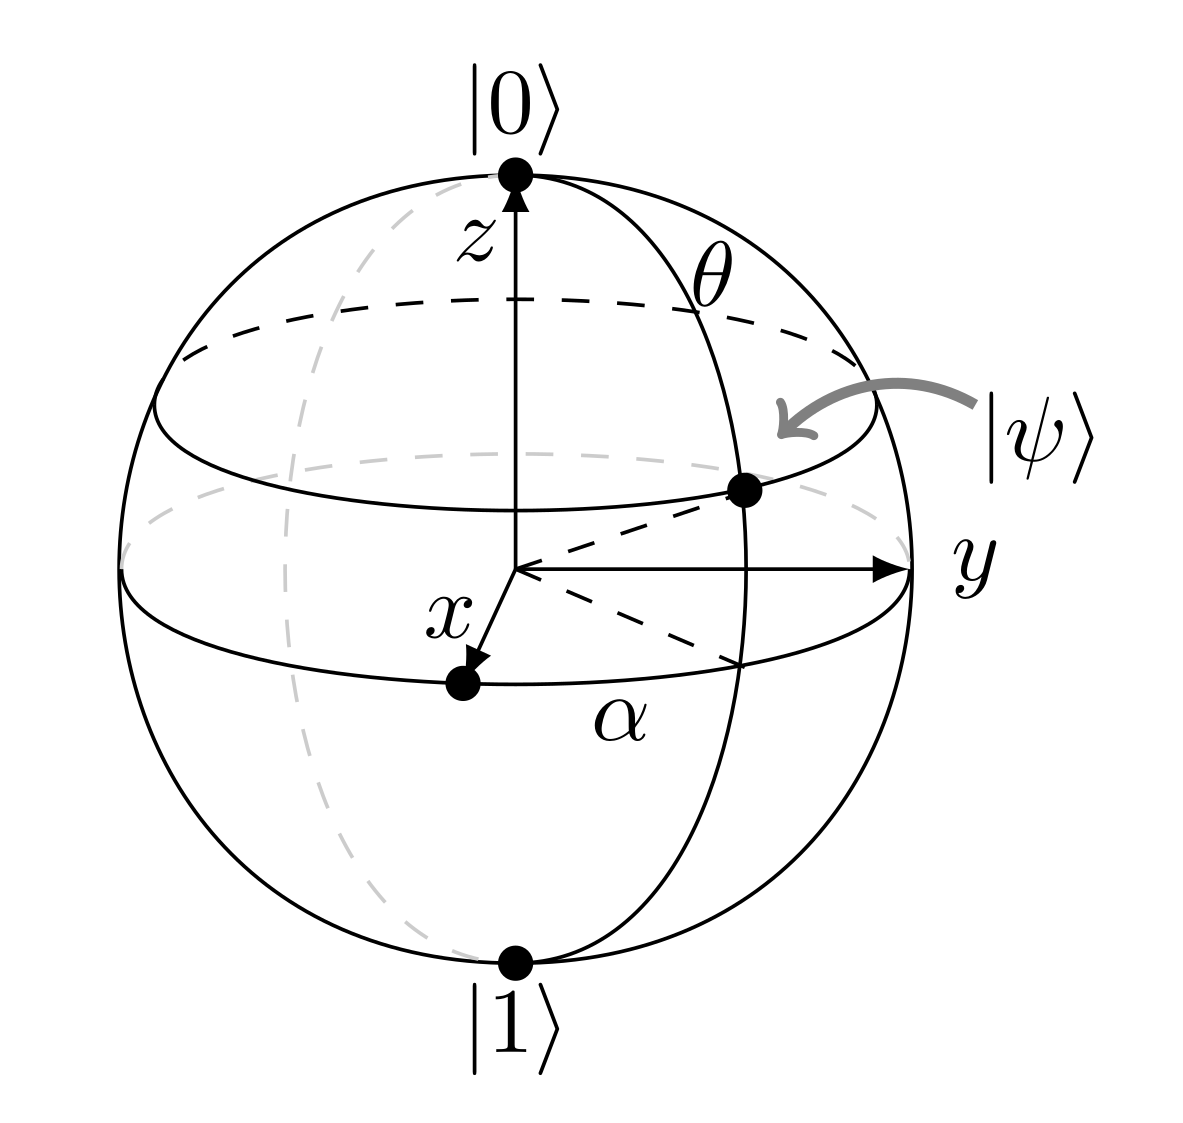
\includegraphics[width=0.5\textwidth]{./figures/bloch.png}
	\caption{Bloch Sphere}
	\label{fig:Bloch Sphere}
\end{figure}

The action of Pauli $Z$ from \eqref{eq:pauli} on the block sphere is.
\begin{dmath*}
	Z \ket{\psi} = Z \ket{\psi} 
	= e^{i \beta} \left(\cos \frac{\theta}{2} \ket{0} - e^{i \alpha} \sin \frac{\theta}{2} \ket{1}\right)
	= e^{i \beta} \left(\cos \frac{\theta}{2} \ket{0} + e^{i \alpha + \pi} \sin \frac{\theta}{2} \ket{1}\right)
\end{dmath*}
It transforms $(\theta, \alpha)$ to $(\theta, \alpha + \pi)$, which is rotation by $\pi$ on $z$ axis.
By similar arguments, we can show Pauli $X, Y$ in \eqref{eq:pauli} correspond to the rotations of $\pi$ along the $x, y$ axis.
It turns out that unitary operations on a single qubit are precisely the rotations on Bloch sphere.

\begin{theorem}[Unitaries on Bloch Sphere]\label{th:unitary-bloch}
	The actions of single-qubit unitary matrices is equivalent to rotation (represented by $SO(3)$) in the Bloch sphere.
\end{theorem}
This theorem is excercise 4.6 from \cite{Nielsen_Chuang_2010}.


\subsection{Measurement}\label{sec:measurement}

Our discussion of measurement is breif and only for the sake of completeness. 
For more details see chapter 2.2 and 4.4 of \cite{Nielsen_Chuang_2010}.

Recall that a positive semidefinite projector is a Hermitian matrix $M$ such that $M^2 = M$ and $\bra{\psi} M \ket{\psi} \geq 0$ for any $\ket{\psi}$. 
Using spectral theorem, we can show that each positive semidefinite projector $M$ can be written as
$$M = \sum_{i} c_i\ket{v_{i}} \bra{v_{i}}, \quad c_i \in \{0, 1\}$$
where $\ket{v_{i}}$ is a set of orthonormal basis of $\mathbb{C}^2$.
That is, the eigenvalues of a positive semidefinite projector are either 0 or 1. 

Let $\mathcal{M} = \{M_1, M_2, \cdots, M_n\}$ be a set of positive semidefinite projectors $V \rightarrow V$ such that $\sum_{i=1}^n M_i = I$. 
Each of $M_i$ is called an observable of the measurement $\mathcal{M}$.
Given a state $\kp$, the probability of obtaining the outcome $i$ is $\bra{\psi} M_i \ket{\psi}$, and the post-measurement state is $\frac{M_i \ket{\psi}}{\sqrt{\bra{\psi} M_i \ket{\psi}}}$.

This principle of obtaining probabilistic outcomes from measurement is called the Born rule.

From Born rule, we see $\kp$ and $e^{i\pi \theta} \kp$ are indistinguishable for any $\theta \in \mathbb{R}$, since 
$$
\bra{\psi} M_i \ket{\psi} = \bra{\psi} e^{-i\pi \theta} M_i e^{i\pi \theta} \ket{\psi}
$$


\subsection{Univeral Gates}

In the effort to build quantum computers one task is especially important: to find some small sets of unitary matrices that can effectively simulate any unitary operations.
These unitary matrices are called universal gates.

Let us first concentrate on the single-qubit unitary operations.
There are infinitely many single qubit unitary operations, making it impossible to exactly synthesize any arbitrary operation with a finite set of gates. 
\footnote{On classical computers, it is well known that NAND gate alone is sufficient to implement any Boolean function \cite{sheffer1913set}.}
Therefore, we relax our goal to find a finite set of gates that can approximate any single qubit unitary operation to arbitrary precision in the sense defined below. 

\begin{definition}[Error of approximation]
	If $U$ is the unitary operation we wish to implement while $V$ is the actual implementation in practice. 
	The \emph{error} of approximation is defined as  
	\begin{equation}
		E(U, V) = \max_{\ket{\psi}} \frac{\| (U - V) \ket{\psi} \|}{\| \ket{\psi} \|}.
	\end{equation}
\end{definition}

This definition of error has two important properties which fits our intuitions for errors. 
\begin{enumerate}
	\item Let $\ket{\psi}$ be our initial state. If $E(U, V)$ is small, the probability of obtaining different measurement outcome from $U \kp$ and $V \kp$ is small;
	\item accumulated error satisfies triangular inequality, that is 
		$$
			E(U_1 U_2, V_1, V_2) \leq E(U_1, V_1) + E(U_2, V_2)
		$$
\end{enumerate}

Their proofs are presented in the appendix \ref{sec:error}.

With the proper definition for error, we can settle the definition of univera;l gate.
\begin{definition}[Universal Gate]
A set of quantum gates is called \emph{universal} if any unitary operation can be aproximated with arbitraily small error by a finite sequence of gates from the set.
\end{definition}

\subsubsection{Universality of Hadamard and T Gates and CNOT}

An important set of universal gate which we discuss in detail here is Hadamard + T gate. 
Where Hadamard gate $H$ and T gate $T$ are defined as
\begin{equation*}
		H = \frac{1}{\sqrt{2}} \begin{pmatrix}
		1 & 1\\
		1 & -1
		\end{pmatrix}, \quad T = \begin{pmatrix}
		1 & 0\\
		0 & e^{i\pi/4}
		\end{pmatrix}.
\end{equation*}

\begin{remark}
	Note that both of $T$ and $H$ are unitary, and $T^4 = Z$ and $HZH = X$.
\end{remark}

\begin{theorem}
	The set $\{H, T\}$ is a universal gate set for single qubit unitary operations.
\end{theorem}

\begin{proof}
	We can write
	$$
	T = \cos \frac{\pi}{8} I - i \sin \frac{\pi}{8} Z, \quad H = \frac{1}{\sqrt{2}} (X + Z).
	$$
	where $X, Z$ are the Pauli X and Z operators, respectively. 
	Calculation shows that 
	$$
	THTH = \cos^2\frac{\pi}{8} I - i \sin \frac{\pi}{8} \left( \cos \frac{\pi}{8} (X + Z) + \sin \frac{\pi}{8} Y \right),
	$$
	This is rotation along the axis $(\cos\frac{\pi}{8}, \sin\frac{\pi}{8}, \cos\frac{\pi}{8})$ through an angle $\theta$ defined by $\cos \frac{\theta}{2} = \cos^2 \frac{\pi}{8}$.
	We can show that $\theta$ is a irrational multiple of $\pi$\footnote{See \cite{boykin1999} and section 4.5.3 of \cite{Nielsen_Chuang_2010}. }.
	Therefore repeated applications of $THTH$ can approximate any rotation along the axis $(\cos\frac{\pi}{8}, \sin\frac{\pi}{8}, \cos\frac{\pi}{8})$ to arbitrary precision.

	By the same calculation we can show that $HTHT$ is a rotation along the axis $(\cos\frac{\pi}{8}, -\sin\frac{\pi}{8}, \cos\frac{\pi}{8})$ through the same angle $\theta$. 
	Repeated applications of $HTHT$ can approximate any rotation along the axis $(\cos\frac{\pi}{8}, -\sin\frac{\pi}{8}, \cos\frac{\pi}{8})$ to arbitrary precision.

	As shown in the appendix, any single qubit unitary $U$ can be represented as 
	$$
	U = R_{\hat{n}}(\alpha) R_{\hat{m}}(\beta) R_{\hat{n}}(\gamma),
	$$
	where $\hat{n}$ and $\hat{m}$ are two non-parallel axes, and $R_{\hat{n}}(\alpha)$ denotes the rotation along axis $\hat{n}$ through angle $\alpha$.

	Previous paragraphs shows that for any $\epsilon > 0$, $H$ and $T$ can be used to approximate generate $V_1, V_2, V_3$ such that $E(R_{\hat{n}}(\alpha), V_1) < \epsilon$, $E(R_{\hat{m}}(\beta), V_2) < \epsilon$ and $E(R_{\hat{n}}(\gamma), V_3) < \epsilon$.
	Applying proposition \ref{prop:cumulation-of-error} we see $E(U, V_1 V_2 V_3) < 3 \epsilon$, proving the universality of $H$ and $T$.
\end{proof}

So $H$ and $T$ gates can approximate any single qubit unitary operation.
The surprising fact is that by adding one more gate, CNOT, they can be used to approximate any unitary operation on any number of qubits. 

\begin{theorem}
	Single qubit gates together with CNOT gate is a universal gate set for quantum computation.
\end{theorem}

\begin{proof}
	The detailed proof can be found here \cite{barenco1995elementary}.
	The gist of the proof is two parts 
	\begin{enumerate}
		\item any multi-qubit unitary operations can be decomposed into two-body unitary operations via Gaussian elimination. \footnote{By two-body unitary operation we mean a unitary operation that acts non-trivially on only a 2-dimensional subspace.} 
		\item any two-body unitary operation can be implemented by CNOT and single qubit gates.
	\end{enumerate}
\end{proof}


